\documentclass{protokol}

\usepackage[czech]{babel}
\usepackage[utf8]{inputenc}
\usepackage{icomma}

% Plovouci bloky (obrazky, tabulky)
\usepackage{floatrow}
\floatsetup[table]{capposition=top}
\floatsetup[figure]{frameset={\fboxsep16pt}}
\usepackage{subcaption}

% Tabulky
\usepackage{tabu}
\usepackage{booktabs}
\usepackage{csvsimple}
\usepackage{multirow}
\usepackage{multicol}

% Jednotky
\usepackage{siunitx}
\sisetup{
	locale               = DE,
	inter-unit-product   = \ensuremath{{}\cdot{}},
	list-units           = single,
	list-separator       = {; },
	list-final-separator = \text{ a },
	list-pair-separator  = \text{ a },
	range-phrase         = \text{ až },
	range-units          = single,
	separate-uncertainty = true,
}
\usepackage{amsmath}

% Obvody
\usepackage{circuitikz}

% Obrazky a grafy
% \usepackage{graphicx}
\graphicspath{
	{img/}
	{plots/}
	{build/plots/}
}
\usepackage{epstopdf}
\epstopdfsetup{outdir=./build/plots/}

\usepackage[backend=biber]{biblatex}
\addbibresource{references.bib}

\jmenopraktika={Experimentální metody I}       % jmeno predmetu
\jmeno={Radek Horňák, Jan Slaný, Lukáš Vrána}  % jmeno mericiho
\obor={F}                                      % zkratka studovaneho oboru
\skupina={Čt 15:00}                            % doba vyuky seminarni skupiny
\rocnik={IV}
\semestr={I}

\cisloulohy={01}
\jmenoulohy={Vektorový síťový analyzátor}

\datum={22. září 2021}                  % datum mereni ulohy
\tlak={}% [hPa]
\teplota={}% [C]
\vlhkost={}% [%]

\newcommand\sparam{S}
\newcommand\male{m}
\newcommand\female{f}
\newcommand\permitfree{\varepsilon_0}
\newcommand\permitrel{\varepsilon_r}
\newcommand\permeabfree{\mu_0}
\newcommand\freq{f}
\newcommand\impedance{Z}
\newcommand\resistance{R}
\newcommand\inductance{L}
\newcommand\capacitance{C}

\newcommand\connector[2]{#1 -- #2}
\newcommand\connectord[3]{#1 -- #2\\ #3}
\tikzset{
	connector/.style={
		draw,
		align=center,
		minimum width=4cm,
		minimum height=1.5cm}
}

\begin{document}
\headernoenv

\section{Úvod}
Elektrické obvody pracující na nízkých frekvencích,
jejichž rozměry jsou malé oproti vlnové délce signálu,
mají v~každém bodě jasně definované napětí a proud.
Díky malým rozměrům je v~nich zároveň zanedbatelné fázové zpoždění
mezi jednotlivými body v~obvodu.
Tyto vlastnosti však obecně neplatí pro vysokofrekvenční obvody.
K~jejich analýze je potřeba přistupovat odlišným způsobem,
než jaký se využívá pro nízkofrekvenční obvody \cite{pozar}.
V~této úloze budeme zabývat vektorovým síťovým analyzátorem,
který je vhodný pro měření parametrů vysokofrekvenčních obvodů.

\section{Teorie}

\subsection{Vektorový síťový analyzátor}

Pro označení vektorového síťového analyzátoru budeme z~anglického
vector network analyzer používat zkratku VNA.
VNA je zpravidla dvoukanálový mikrovlnný měřící přístroj,
pomocí nějž se měří rozptylové parametry elektrických obvodů
s~různými prvky pro vysokofrekvenční aplikace.
VNA je konstruován na měření velikosti a fáze prošlého a odraženého vlnění
z~měřeného obvodu,
který je obecně označován zkratkou DUT z~anglického device 
under test \cite{pozar}.
VNA obsahuje zdroj signálu o~známých frekvencích a soustavu přijímačů,
které měří změny v~signálu způsobené připojeným DUT.
Schéma funkce přístroje je na obr.~\ref{VNA}.
Vygenerovaný signál postupuje směrem k~DUT.
Část signálu se na vstupu DUT odrazí zpět, část projde k~výstupnímu portu.
Přijímače poté porovnávají výsledný signál na ně dopadající
se signálem vygenerovaným ve zdroji.
Výsledek je poté počítačově zpracován a zobrazen na displeji.
Výstupem měření VNA jsou prvky rozptylové matice.

\begin{figure}[b]
	\centering
	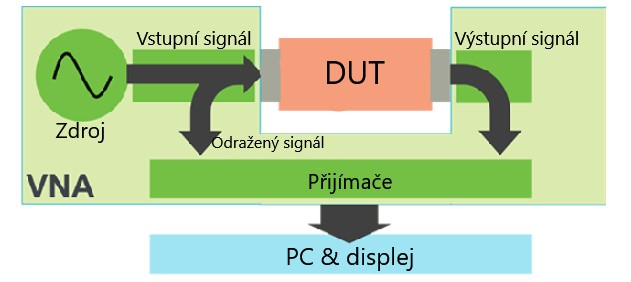
\includegraphics[width=100mm,]{network-analyzer-diagram}
	\caption{Princip funkce VNA, převzato z~\cite{tektronix} a upraveno.}
	\label{VNA}
\end{figure}


\subsection{Rozptylová matice}

Přímé měření napětí a proudů v~mikrovlnných obvodech není vhodné,
jelikož naměřené hodnoty obsahují velikost a fázi postupující vlny
v~daném směru nebo vlny stojaté.
Je potřeba brát v~potaz dopadající, prošlé i odražené vlny.
Proto zavádíme pojem rozptylová matice, která se označuje 
jako $(S)$ matice \cite{pozar}.
Rozptylová matice poskytuje kompletní popis obvodu s~$N$ svorkami,
konkrétně vytváří vztah mezi vlněním dopadajícím na svorky
a vlněním na svorkách odraženým.
Pro některé prvky je možné $(S)$ matice dopočítat,
ovšem jednodušší způsob je prvky matice přímo změřit pomocí VNA.
$(S)$ matice je definovaná jako:
\[
\begin{pmatrix}
	U^-
\end{pmatrix}
=
\begin{pmatrix}
	S~\end{pmatrix}
%
\begin{pmatrix}
	U^+
\end{pmatrix}
,\]
kde $U^+$ a $U^-$ jsou amplitudy dopadajícího a odraženého napětí
(v~tomto pořadí) \cite{pozar}.

Pro obvod s~$N$ svorkami má $(S)$ matice tvar:
\[
\begin{pmatrix}
	U_1^-     \\
	U_2^-		\\
	\vdots	\\
	U_N^-
\end{pmatrix}
=
\begin{pmatrix}
	S_{11} & S_{12} & \dots & S_{1N}   \\
	S_{21} &		& 		& \vdots	\\
	\vdots &		& 		& \vdots	\\
	S_{N1} & \dots	& \dots & S_{NN} 	\\
\end{pmatrix}
%
\begin{pmatrix}
	U_1^+     \\
	U_2^+		\\
	\vdots	\\
	U_N^+
\end{pmatrix}
.\]

Pro obvod s~dvěma svorkami tedy bude $(S)$ matice řádu 2.
V~ní prvek $S_{11}$ vyjadřuje odražený signál na vstupu,
$S_{22}$ odraz na výstupu, $S_{21}$ je transmisní prvek ze vstupu na výstup
a $S_{12}$ je transmisní prvek z~výstupu na vstup.

\subsection{Impedanční a admitanční matice}

Impedance $Z$ je komplexní veličinou a je definovaná jako poměr napětí a proudu:
\begin{equation}
	Z~= \frac{U}{I} \:.
\end{equation}

Admitance $Y$ je převrácenou hodnotou impedance, tedy platí:
\begin{equation}
	Y = \frac{1}{Z} \:.
\end{equation}

Impedanční matice $(Z)$ mikrovlnného obvodu s~$N$ svorkami
udává vztah mezi napětími a proudy následovně:
\[
\begin{pmatrix}
	V_1     \\
	V_2		\\
	\vdots	\\
	V_N
\end{pmatrix}
=
\begin{pmatrix}
	Z_{11} & Z_{12} & \dots & Z_{1N}   \\
	Z_{21} &		& 		& \vdots	\\
	\vdots &		& 		& \vdots	\\
	Z_{N1} & \dots	& \dots & Z_{NN} 	\\
\end{pmatrix}
%
\begin{pmatrix}
	I_1     \\
	I_2		\\
	\vdots	\\
	I_N
\end{pmatrix}
.\]

Admitanční matice $(Y)$ je definovaná jako
\[
\begin{pmatrix}
	Y
\end{pmatrix}
=
\begin{pmatrix}
	Z~\end{pmatrix}^{-1}
,\]

což pro obvod s~$N$ svorkami můžeme rozepsat ve tvaru

\[
\begin{pmatrix}
	I_1     \\
	I_2		\\
	\vdots	\\
	I_N
\end{pmatrix}
=
\begin{pmatrix}
	Y_{11} & Y_{12} & \dots & Y_{1N}   \\
	Y_{21} &		& 		& \vdots	\\
	\vdots &		& 		& \vdots	\\
	Y_{N1} & \dots	& \dots & Y_{NN} 	\\
\end{pmatrix}
%
\begin{pmatrix}
	V_1     \\
	V_2		\\
	\vdots	\\
	V_N
\end{pmatrix}
.\]

\subsection{Výpočet impedanční a admitanční matice z~rozptylové matice}

Impedanční matici $(Z)$ můžeme vyjádřit pomocí rozptylové matice $(S)$ jako:
\[
\begin{pmatrix}
	Z~\end{pmatrix}
=
[\begin{pmatrix}
	A~\end{pmatrix}
+
\begin{pmatrix}
	S~\end{pmatrix}]
%
[\begin{pmatrix}
	A~\end{pmatrix}
-
\begin{pmatrix}
	S~\end{pmatrix}]^{-1}
,\]
kde $(A)$ je jednotková matice.
\bigskip

Obdobně můžeme pomocí rozptylové matice $(S)$ a jednotkové matice $(A)$
vyjádřit i admitanční matici jako:
\[
\begin{pmatrix}
	Y
\end{pmatrix}
=
[\begin{pmatrix}
	A~\end{pmatrix}
-
\begin{pmatrix}
	S~\end{pmatrix}]
%
[\begin{pmatrix}
	A~\end{pmatrix}
+
\begin{pmatrix}
	S~\end{pmatrix}]^{-1}
.\]

\subsection{Transmisní matice}
Při měření je v~obvodu zpravidla zapojeno více prvků.
Proto je vhodné zavést transmisní matici $(T)$ pro každý z~prvků.
U~dvojbranů je matice $(T)$ řádu 2 a má tvar
\[
\begin{pmatrix}
	A~& B  \\
	C &	D  \\
\end{pmatrix}
.\]

V~nejjednodušším obvodu se dvěma prvky je mezi celkovou transmisní
maticí $(ABCD)$, transmisní maticí prvního prvku $(A_1B_1C_1D_1)$
a transmisní maticí druhého prvku $(A_2B_2C_2D_2)$ vztah následující:

\[
\begin{pmatrix}
	A~& B  \\
	C &	D  \\
\end{pmatrix}
=
\begin{pmatrix}
	A_1 & B_1  \\
	C_1 & D_1  \\
\end{pmatrix}
%
\begin{pmatrix}
	A_2 & B_2  \\
	C_2 & D_2  \\
\end{pmatrix}
.\]

Dále platí:

\begin{equation}
	A~= \frac{(1+S_{11})(1-S_{22})+S_{12}S_{21}}{2S_{21}},
	\label{eq:A}
\end{equation}

\begin{equation}
	B = Z_0 \frac{(1+S_{11})(1+S_{22})-S_{12}S_{21}}{2S_{21}},
	\label{eq:B}
\end{equation}

\begin{equation}
	C = \frac{1}{Z_0} \frac{(1-S_{11})(1-S_{22})-S_{12}S_{21}}{2S_{21}},
	\label{eq:C}
\end{equation}

\begin{equation}
	D = \frac{(1-S_{11})(1+S_{22})+S_{12}S_{21}}{2S_{21}},
	\label{eq:D}
\end{equation}
kde $\impedance_{0}$ je charakteristická impedance.

Zpětný přepočet $ABCD$ prvků na $S_{11}$ a $S_{21}$ lze provést jako

\begin{equation}
	S_{11} = \frac{A+B/Z_0-CZ_0-D}{A+B/Z_0+CZ_0+D},
	\label{eq:s11}
\end{equation}

\begin{equation}
	S_{21} = \frac{2}{A+B/Z_0+CZ_0+D}.
	\label{eq:s21}
\end{equation}

\subsection{Výpočet impedance z~$\sparam_{11}$ v~případě jednobranu}
V~případě jednobranu měříme pouze prvek $\sparam_{11}$, impedanci $\impedance$ 
lze z~něj dopočítat ze vztahu

\begin{equation}
	\impedance = \impedance_{0}\frac{1+\sparam_{11}}{1-\sparam{11}}.
	\label{eq:Z}
\end{equation}


\subsection{Typy konektorů}
V~tomto praktiku budeme měřit různá zapojení koaxiálních konektorů typu
SMA, BNC a N s~impedancí 50~$\Omega$.

SubMiniature Type-A neboli SMA konektor je jedním z~nejpoužívanějších
mikrovlnných konektorů. Je zobrazený na obr.~\ref{SMA}.
Vnitřní průměry jeho koaxiálního vedení jsou 4,1~mm a 1,27~mm,
funkci izolantu v~něm plní teflon.
Spojení se zajišťuje pomocí šroubovacího mechanismu.
Obecně se uvádí, že je vhodný až do frekvence 18~GHz \cite{rfhandbook}.

Bayonet Neill Concelman, někdy nazývaný Bayonet Navel Connector,
zkráceně BNC, je konektor vyvinutý ve čtyřicátých letech dvacátého století.
Jeho charakteristikou je bajonetový mechanismus spojení.
Tento mechanismus je tvořen dvěma výstupky na samičím konektoru
a drážkou se spirálou a vybráním na převlečné části samčího konektoru,
viz obr.~\ref{BNC}.
Umožňuje rychlé a spolehlivé spojení nasunutím a pootočením převlečné
části o~90$^{\circ}$ \cite{czwiki}.
Konektor je vhodný až do frekvence 11~GHz \cite{rfhandbook}.

Konektor typu N, pojmenovaný po jeho vynálezci Paulu Neillovi,
vznikl ve čtyřicátých letech dvacátého století.
Jedná se o~konektor s~klasickým šroubovacím mechanismem.
Využívá se při aplikacích, kde frekvence nepřesahuje 11~GHz \cite{rfhandbook}.
Je zobrazený na obr.~\ref{N}.

\begin{center}
	\captionsetup{justification=centering}
	\begin{minipage}{0.32\textwidth}
		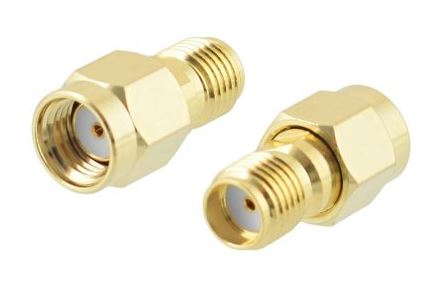
\includegraphics[width=\textwidth]{connector-sma}
		\captionof{figure}{SMA konektor, převzato z~\cite{gme}}
		\label{SMA}
	\end{minipage}
	\begin{minipage}{0.40\linewidth}
		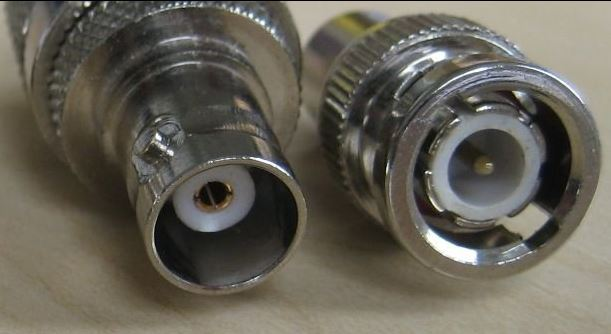
\includegraphics[width=\linewidth]{connector-bnc}
		\captionof{figure}{BNC konektor, převzato z~\cite{czwiki}}
		\label{BNC}
	\end{minipage}
	\begin{minipage}{0.29\textwidth}
		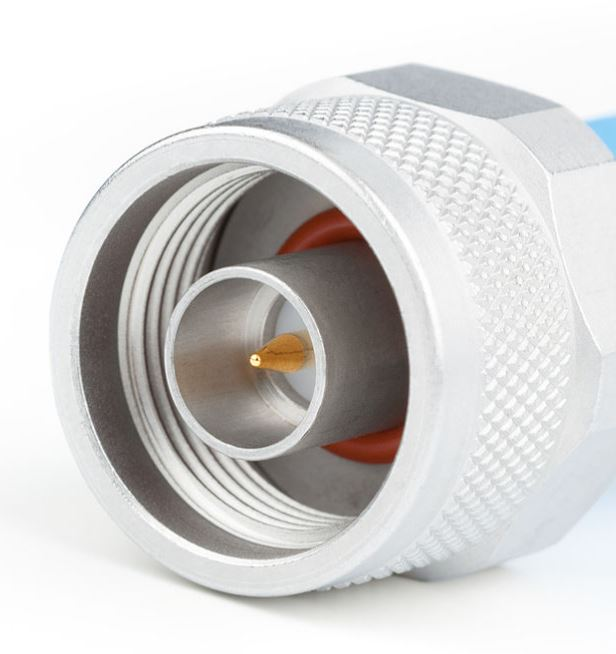
\includegraphics[width=\textwidth]{connector-n}
		\captionof{figure}{N konektor, převzato z~\cite{enwiki}}
		\label{N}
	\end{minipage}
\end{center}

\section{Praktická část}
\subsection{Kalibrace přístroje}
K~měření budeme používat vektorový síťový analyzátor Rohde \& Schwarz ZVL,
který měří v~rozsahu 9~kHz až 13,6~GHz.
Měřený prvek se k~přístroji připojuje pomocí testovacích kabelů s~SMA konektory.
Tyto kabely však nejsou dokonalé a mění parametry celého systému.
Před samotným měřením je tedy potřeba přístroj s~kabely nakalibrovat.
Pro kalibraci jednoho portu potřebujeme tři různé impedance.
Z~praktických důvodů se volí známé impedance při třech situacích -- zkrat (short),
otevřený obvod (open) a přizpůsobený obvod (match).
Nejvhodnějším způsobem kalibrace je využití kalibračního členu,
pomocí nějž lze jednoduše výše zmíněné impedance vytvořit.
K~dispozici máme kalibrační člen Rohde \& Schwarz ZV-Z135,
k~němuž jsou dodávány i korekce, které už máme ve VNA nahrané.
Kalibraci je potřeba provést na každém portu zvlášť i na obou portech současně.
Zároveň je potřeba kalibraci provést pečlivě,
protože nedbalá kalibrace způsobená špatně připojeným kalibračním členem
by mohla ovlivnit všechna následně naměřená data.

První připojíme port 1 jako otevřený obvod.
Veškerý signál by se měl odrazit, čemuž odpovídá $S_{11}$ = 0~dB.
Další na řadě je zkrat na portu 1.
Na zkratu se nemá výkon kde ztratit,
takže opět dochází k~úplnému odrazu a znovu platí, že $S_{11}$ = 0~dB.
Zbývá připojení portu 1 na přizpůsobenou impedanci.
V~tomto případě by se měl ideálně veškerý signál absorbovat,
tedy $S_{11}$ by měla být co nejnižší.
U~frekvence 10~GHz je $S_{11}$ přibližně $-25$~dB,
minimum $S_{11}$ je okolo $-50$~dB. Tyto hodnoty považujeme 
za dostatečně nízké.

Kalibrace druhého portu probíhá obdobně,
přičemž se místo $S_{11}$ měří $S_{22}$.
Pro otevřený obvod, zkrat i přizpůsobený obvod dává přístroj prakticky
stejné hodnoty $S_{22}$ na portu 2 jako jsme naměřili pro $S_{11}$ na portu 1.

Posledním krokem je kalibrace obou portů současně nazývaná
jako zapojení through.
Přístroj měří $S_{21}$, která je podle očekávání kolem 0~dB.
Tím je kalibrace hotová.

Z~předpokladu symetrie budeme dále uvažovat rovnosti
$S_{11}$ = $S_{22}$ a $S_{21}$ = $S_{12}$.

\subsection{1. měření: zlatý konektor SMA\female}
Jako první měříme konektor SMA, který má z~obou stran samičí vstup (značíme f),
schéma zapojení je na obr.~\ref{fig:exp1}.
Konektor je zlaté barvy (index $_\text{Z}$), což rozlišuje pouze z~důvodu,
že budeme srovnávat dva konektory stejného typu lišící se barvou.
Výsledné zapojení tedy označíme jako (SMAf/SMAf)$_\text{Z}$.
Obdobné značení budeme využívat i nadále.
Z~obr.~\ref{fig:01-sparam} je vidět,
že v~GHz frekvencích se na konektoru začíná signál odrážet (viz $\sparam_{11}$),
a na~frekvencích blížících se \SI{10}{\giga\hertz} je signál zeslaben téměř
o~\SI{0.5}{\decibel}.

\begin{figure}[h]
	\centering
	\begin{circuitikz}
		\node[connector] (con1) at (0,0)
		{\connectord{SMA\female}{SMA\female}{zlatý}};
		\draw (con1.west) to[short, -o] +(-1,0);
		\draw (con1.east) to[short, -o] +(1,0);
	\end{circuitikz}
	\caption{Schéma zapojení 1. měření.}
	\label{fig:exp1}
\end{figure}

\subsection{2. měření: stříbrný konektor SMA\female}
Měříme opět konektor (SMAf/SMAf)$_\text{S}$, avšak nyní je konektor
ve stříbrné barvě (index $_\text{S}$).
Schéma zapojení je na obr.~\ref{fig:exp2}.
V~porovnání s~konektorem ve zlaté barvě z~prvního měření
je u~stříbrného
z~$S_{11}$ stříbrného konektoru na obr.~\ref{fig:02-sparam} má podobný průběh 
jako u~zlatého konektoru.
U~$S_{21}$ je vidět oproti zlatému konektoru menší útlum.
Může se tedy jednat o~kvalitnější součástku,
nebo je lepší průchod signálu způsoben preciznějším dotažením.

\begin{figure}[h]
	\centering
	\begin{circuitikz}
		\node[connector] (con1) at (0,0)
		{\connectord{SMA\female}{SMA\female}{stříbrný}};
		\draw (con1.west) to[short, -o] +(-1,0);
		\draw (con1.east) to[short, -o] +(1,0);
	\end{circuitikz}
	\caption{Schéma zapojení 2. měření.}
	\label{fig:exp2}
\end{figure}

\begin{figure}[htp]
	\centering
	\input{plots/data01-s11}
	\input{plots/data01-s21}
	\caption{Naměřené hodnoty parametrů $\sparam_{11}$ a~$\sparam_{21}$
		zlatého konektoru SMA\female.}
	\label{fig:01-sparam}
\end{figure}

\begin{figure}[htp]
	\centering
	\input{plots/data02-s11}
	\input{plots/data02-s21}
	\caption{Naměřené hodnoty parametrů $\sparam_{11}$ a~$\sparam_{21}$
		stříbrného konektoru SMA\female.}
	\label{fig:02-sparam}
\end{figure}

\clearpage
\subsection{3. měření: trojice konektorů SMA}
Měříme zapojení 
(SMAf/SMAf)$_\text{Z}$---(SMAm/SMAm)$_\text{Z}$---(SMAf/SMAf)$_\text{S}$,
kde m značí samčí vstup.
Schéma zapojení je na obr.~\ref{fig:exp3}.
Úkolem je dopočítat matice prostředního konektoru (SMAm/SMAm)$_\text{Z}$,
matice pro zbylé konektory známe z~předchozích měření. Hodnoty $\sparam_{11}$ 
a~$\sparam_{21}$ pro naměřenou trojici konektorů vidíme na obr.~
\ref{fig:03-sparam} a dopočítané 
hodnoty pomocí rovnic \eqref{eq:A} až \eqref{eq:s21} jsou vyneseny do grafu na 
obr.~\ref{fig:03-result-sparam}. Z~dopočítaných hodnot vychází, že konektor by 
měl při frekvencích $>\SI{1}{\giga\hertz}$ zesilovat signál. Jelikož se jedná 
pouze o~velmi nízké hodnoty, vysvětlením může být šum nebo nedokonalé dotažení 
spojů, na které je vysokofrekvenční měření citlivé.

\begin{figure}[h]
	\centering
	\begin{circuitikz}
		\node[connector] (con1) at (-4,0)
		{\connectord{SMA\female}{SMA\female}{zlatý}};
		\node[connector] (con2) at (0,0)
		{\connectord{SMA\male}{SMA\male}{zlatý}};
		\node[connector] (con3) at (4,0)
		{\connectord{SMA\female}{SMA\female}{stříbrný}};
		\draw (con1.west) to[short, -o] +(-1,0);
		\draw (con3.east) to[short, -o] +(1,0);
	\end{circuitikz}
	\caption{Schéma zapojení 3. měření.}
	\label{fig:exp3}
\end{figure}

\subsection{4. měření: dvojice redukcí \connector{SMA\female}{BNC}}
Máme zapojení (SMAf/BNCm)---(BNCf/SMAf),
jeho schéma je vidět na obr.~\ref{fig:exp4}.
Jelikož nedokážeme zapojit ani jeden z~těchto konektorů samostatně
a chceme znát matici jednoho z~nich,
konektory budeme považovat za identické a výslednou matici
jednoho konektoru určíme jako odmocninu z~naměřené matice.
Naměřené hodnoty parametrů $\sparam_{11}$ a~$\sparam_{21}$ pro celé zapojení 
jsou vyneseny do grafů na obr.~\ref{fig:04-sparam} a vypočítané hodnoty jsou na 
obr.~\ref{fig:04-result-sparam}. V~porovnání s~SMA konektory dochází u~těchto 
redukcí k~většímu útlumu, a to až o~$\SI{2}{dB}$ při $\SI{5}{\giga\hertz}$. 
Spojka je vhodná pro použití do $\SI{1}{\giga\hertz}$.

\begin{figure}[h]
	\centering
	\begin{circuitikz}
		\node[connector] (con1) at (-2,0)
		{\connector{SMA\female}{BNC\male}};
		\node[connector] (con2) at (2,0)
		{\connector{BNC\female}{SMA\female}};
		\draw (con1.west) to[short, -o] +(-1,0);
		\draw (con2.east) to[short, -o] +(1,0);
	\end{circuitikz}
	\caption{Schéma zapojení 4. měření.}
	\label{fig:exp4}
\end{figure}

\subsection{5.měření: průchodka BNC\female}
Ze zapojení (SMAf/BNCm)---(BNCf/BNCf)---(BNCm/SMAf),
jehož schéma je vidět na obr.~\ref{fig:exp5},
chceme nalézt parametry průchodky (BNCf/BNCf).
Výpočet lze provézt díky znalosti výsledků z~měření 4. Naměřené hodnoty 
parametrů $\sparam_{11}$ a~$\sparam_{21}$ je na obr.~\ref{fig:05-sparam} a 
vypočítané hodnoty parametrů $\sparam_{11}$ a~$\sparam_{21}$ pro průchodku 
BNC\female jsou na obr.~\ref{fig:05-result-sparam}. Opět vidíme, že pro 
frekvence nad $\SI{1}{\giga\hertz}$ nejsou tyto konektory vhodné.

\begin{figure}[h]
	\centering
	\begin{circuitikz}
		\node[connector] (con1) at (-4,0)
		{\connector{SMA\female}{BNC\male}};
		\node[connector] (con2) at (0,0)
		{\connector{BNC\female}{BNC\female}};
		\node[connector] (con3) at (4,0)
		{\connector{BNC\male}{SMA\female}};
		\draw (con1.west) to[short, -o] +(-1,0);
		\draw (con3.east) to[short, -o] +(1,0);
	\end{circuitikz}
	\caption{Schéma zapojení 5. měření.}
	\label{fig:exp5}
\end{figure}

\begin{figure}[p]
	\centering
	\input{plots/data03-s11}
	\input{plots/data03-s21}
	\caption{Naměřené hodnoty parametrů $\sparam_{11}$ a~$\sparam_{21}$
		trojice konektorů SMA.}
	\label{fig:03-sparam}
\end{figure}

\begin{figure}[p]
	\centering
	\input{plots/results03-s11}
	\input{plots/results03-s21}
	\caption{Spočtené hodnoty parametrů $\sparam_{11}$ a~$\sparam_{21}$
		kontektoru SMA\male.}
	\label{fig:03-result-sparam}
\end{figure}

\begin{figure}[p]
	\centering
	\input{plots/data04-s11}
	\input{plots/data04-s21}
	\caption{Naměřené hodnoty parametrů $\sparam_{11}$ a~$\sparam_{21}$
		dvojice redukcí \connector{SMA\female}{BNC}.}
	\label{fig:04-sparam}
\end{figure}

\begin{figure}[p]
	\centering
	\input{plots/results04-s11}
	\input{plots/results04-s21}
	\caption{Spočtené hodnoty parametrů $\sparam_{11}$ a~$\sparam_{21}$
		redukce \connector{SMA\female}{BNC}.}
	\label{fig:04-result-sparam}
\end{figure}

\begin{figure}[p]
	\centering
	\input{plots/data05-s11}
	\input{plots/data05-s21}
	\caption{Naměřené hodnoty parametrů $\sparam_{11}$ a~$\sparam_{21}$
		sestavy redukcí \connector{SMA\female}{BNC} a~průchodky BNC\female.}
	\label{fig:05-sparam}
\end{figure}

\begin{figure}[p]
	\centering
	\input{plots/results05-s11}
	\input{plots/results05-s21}
	\caption{Spočtené hodnoty parametrů $\sparam_{11}$ a~$\sparam_{21}$
		průchodky BNC\female.}
	\label{fig:05-result-sparam}
\end{figure}

\clearpage
\subsection{6. měření: rezonance na T-průchodce BNC}
\newcommand\freelen{d}
Zapojení (SMAf/BNCm)---(BNCf/BNCm/BNCf)---(BNCm/SMAf),
přičemž (BNCf/BNCm/BNCf) je člen ve tvaru T.
Prostřední vstup členu T je zde jako otevřený obvod, viz obr.~\ref{fig:exp6}.
Na otevřeném obvodu dochází k~odrazu signálu a destruktivní interferenci, což 
je vidět na naměřených hodnotách parametrů $\sparam_{11}$ a~$\sparam_{21}$ na 
obr.~\ref{fig:06-sparam}.
Délka prostředního vstupu $d$ je s~frekvencí $f$,
při níž dochází k~destruktivní interferenci, spojena vztahem
\begin{equation}
	d = \frac{(2k+1)}{4f} \frac{1}{\sqrt{\varepsilon_0 \varepsilon_r \mu_0}},
	\label{eq:resonance-length}
\end{equation}
kde k~= 0,1,2,... je řád maxima, $\varepsilon_0$ je permitivita vakua,
$\varepsilon_r = \num{2.25}$ je v~tomto případě relativní permitivita polyethylenu
a $\mu_0$ je permeabilita vakua.

Pro stanovení neznámé délky $\freelen$ přepišme vztah
\eqref{eq:resonance-length} do tvaru:
\begin{align}
	\label{eq:resonance-length-freq}
	f &= \frac{1}{\freelen} \frac{2k+1}{4}
		\frac{1}{\sqrt{\permitfree\permitrel\permeabfree}}
		= ax + b &
	a &= 1/\freelen \\
	& &
	x &= \frac{2k+1}{4}
		\frac{1}{\sqrt{\permitfree\permitrel\permeabfree}}
\end{align}
kde parametry $a$ a $b$ aproximujeme metodou nejmenších čtverců
a~spočteme délku $\freelen = 1/a$.

Destruktivní interference pro $\lambda/4$ nastává při frekvenci 3,33~GHz
s~útlumem 42~dB. Pro $3\lambda/4$ je útlum 36,4~dB na
frekvenci 8,47~GHz.
Délka $d$ spočtená podle vztahu~\eqref{eq:resonance-length-freq} je
\SI{19.4}{\milli\metre}. Odhadovaná délka naměřená ručně posuvným měřítkem je 
$\approx\SI{23}{\milli\metre}$.
% TODO: Calculate uncertainty

\begin{figure}[hb]
	\centering
	\begin{circuitikz}
		\node[connector, minimum height=1.5cm] (con1) at (-4,0)
		{\connector{SMA\female}{BNC\male}};
		\draw (-2,-0.75) -- (2,-0.75) -- (2,0.75) -- (0.75,0.75) -- (0.75,2)
		-- (-0.75,2) -- (-0.75,0.75) -- (-2,0.75) -- cycle;
		\node at (-1.2,0) {BNC\female};
		\node at (0,1.375) {BNC\male};
		\node at (1.2,0) {BNC\female};
		\node[connector, minimum height=1.5cm] (con3) at (4,0)
		{\connector{BNC\male}{SMA\female}};
		\draw (con1.west) to[short, -o] +(-1,0);
		\draw (con3.east) to[short, -o] +(1,0);
	\end{circuitikz}
	\caption{Schéma zapojení 6. měření.}
	\label{fig:exp6}
\end{figure}

\subsection{7. měření: rezonance na T-průchodce s~volným vodičem}
Měříme (SMAf/BNCm)---(BNCf/BNCm + kabel /BNCf)---(BNCm/SMAf).
Zapojení je stejné jako u~měření 6, tentokrát je však na prostřední vstup
T členu připojen kabel neznámé délky, viz obr.~\ref{fig:exp7}. Naměřené hodnoty 
$\sparam_{11}$ a~$\sparam_{21}$ jsou na obr.~\ref{fig:07-sparam}.

Postup je obdobný předchozímu případu. Pro výpočet délky $\freelen$
jsme zvolili minima signálu $\sparam_{21}$ příslušící frekvencím
pod \SI{3e8}{\hertz}, tedy patnáct hodnot.
U~vyšších frekvencí roste nejistota určení polohy minima, jelikož
se prodlužuje krok vzorkování, a proto nebyly uvažovány.

Délka kabelu spočtená výše uvedenou metodou činí
$\freelen = \SI{5.072(4)}{\metre}$.

\begin{figure}[hb]
	\centering
	\begin{circuitikz}
		\node[connector, minimum height=1.5cm] (con1) at (-4,0)
		{\connector{SMA\female}{BNC\male}};
		\draw (-2,-0.75) -- (2,-0.75) -- (2,0.75) -- (0.75,0.75) -- (0.75,2)
		-- (-0.75,2) -- (-0.75,0.75) -- (-2,0.75) -- cycle;
		\node at (-1.2,0) {BNC\female};
		\node at (0,1.375) {BNC\male};
		\node at (1.2,0) {BNC\female};
		\node[connector, minimum height=1.5cm] (con3) at (4,0)
		{\connector{BNC\male}{SMA\female}};
		\draw (0,2) to[short, -o] (0,2.5);
		\draw (con1.west) to[short, -o] +(-1,0);
		\draw (con3.east) to[short, -o] +(1,0);
	\end{circuitikz}
	\caption{Schéma zapojení 7. měření.}
	\label{fig:exp7}
\end{figure}

\begin{figure}[p]
	\centering
	\input{plots/data06-s11}
	\input{plots/data06-s21}
	\caption{Naměřené hodnoty parametrů $\sparam_{11}$ a~$\sparam_{21}$
		sestavy redukcí \connector{SMA\female}{BNC} a~T-průchodky BNC.}
	\label{fig:06-sparam}
\end{figure}
\clearpage

\begin{figure}[p]
	\centering
	\input{plots/data07-s11}
	\input{plots/data07-s21}
	\caption{Naměřené hodnoty parametrů $\sparam_{11}$ a~$\sparam_{21}$
		sestavy redukcí \connector{SMA\female}{BNC}
		a~T-průchodky BNC s~volným vodičem.}
	\label{fig:07-sparam}
\end{figure}

\clearpage
\subsection{8. měření: rezonance na T-průchodce s~vodičem zakončeným terminátorem}
Zapojení (SMAf/BNCm)---(BNCf/BNCm + kabel + terminátor /BNCf)---(BNCm/SMAf)
vychází z~měření 7, ke kabelu je navíc připojen terminátor.

Jelikož impedance terminátoru je shodná s~impedancí vedení,
z~pohledu vstupujícího signálu se jedná o~dvě stejně velké impedance
zapojené vedle sebe.
Dochází tedy k~dělení výkonu rovným dílem mezi obě větve.
Očekáváme proto, že výkon procházejícího signálu bude polovinou výkonu
vstupujícího, což odpovídá poklesu o~zhruba \SI{3.01}{\decibel}.
Jak je patrno z~parametru $\sparam_{21}$ na obr.~\ref{fig:08-sparam},
tento předpoklad je splněn.

\begin{figure}[h]
	\centering
	\begin{circuitikz}
		\node[connector, minimum height=1.5cm] (con1) at (-4,0)
		{\connector{SMA\female}{BNC\male}};
		\draw (-2,-0.75) -- (2,-0.75) -- (2,0.75) -- (0.75,0.75) -- (0.75,2)
		-- (-0.75,2) -- (-0.75,0.75) -- (-2,0.75) -- cycle;
		\node at (-1.2,0) {BNC\female};
		\node at (0,1.375) {BNC\male};
		\node at (1.2,0) {BNC\female};
		\node[connector, minimum height=1.5cm] (con3) at (4,0)
		{\connector{BNC\male}{SMA\female}};
		\node[genericshape, rotate=90] (term) at (0,3.5) {};
		\node at (0.6,3.5) {$\impedance_0$};
		\draw (0,2) -- (term.west);
		\draw (con1.west) to[short, -o] +(-1,0);
		\draw (con3.east) to[short, -o] +(1,0);
	\end{circuitikz}
	\caption{Schéma zapojení 8. měření.}
	\label{fig:exp8}
\end{figure}

\subsection{9. měření: banánkový spoj}
Zapojení (SMAf/BNCm)---(BNCf/banánky m)---(banánky f/BNCf)---(BNCm/SMAf),
přičemž ba\-nán\-ky je koaxiální vedení zapojeno způsobem jádro--jádro a 
stínění--stínění, viz schéma na obr.~\ref{fig:exp9}. Z~obr.~\ref{fig:09-sparam} 
můžeme říct, že do $\SI{0.1}{\giga\hertz}$ je tento typ spoje použitelný. Nad 
$\SI{1}{\giga\hertz}$ je oproti předchozím měřením jiných spojů vidět, že 
banánky vůbec nejsou vhodné pro vysoké frekvence.

\begin{figure}[h]
	\centering
	\begin{circuitikz}
		\node[connector] (con1) at (-5,0)
		{\connector{SMA\female}{BNC\male}};
		\node[connector, minimum width=1.4cm] (con2) at (-2.3,0)
		{BNC\female};
		\node[connector, minimum width=1.4cm] (con3) at (2.3,0)
		{BNC\female};
		\coordinate[yshift=2mm] (n1) at (con2.east) {};
		\coordinate[yshift=0-2mm] (n2) at (con2.east) {};
		\coordinate[yshift=2mm] (n3) at (con3.west) {};
		\coordinate[yshift=0-2mm] (n4) at (con3.west) {};
		\draw (n1) to[short, -o] +(1.4,0);
		\draw (n2) to[short, -*] +(1.4,0);
		\draw (n3) to[short, -o] +(-1.4,0);
		\draw (n4) to[short, -*] +(-1.4,0);
		\node at (0,0.6) {banánky};
		\node[connector] (con4) at (5,0)
		{\connector{BNC\male}{SMA\female}};
		\draw (con1.west) to[short, -o] +(-1,0);
		\draw (con4.east) to[short, -o] +(1,0);
	\end{circuitikz}
	\caption{Schéma zapojení 9. měření.}
	\label{fig:exp9}
\end{figure}

\subsection{10. měření: banánkový spoj s~překřížením}
Vycházíme ze zapojení jako u~měření 9 (SMAf/BNCm)---(BNCf/banánky m)---(banánky 
f/BNCf)---(BNCm/SMAf), přičemž nyní přehozením banánků máme zapojení 
koaxiálního vedení do kříže, tedy jádro--stínění, viz obr.~\ref{fig:exp10}.

Očekáváme horší výsledky než v~měření 9. Na obr.~\ref{fig:10-sparam} pozorujeme 
mizerné hodnoty parametrů $\sparam_{11}$ a~$\sparam_{21}$ na celém spektru 
frekvencí.

\begin{figure}[h]
	\centering
	\begin{circuitikz}
		\node[connector] (con1) at (-5,0)
		{\connector{SMA\female}{BNC\male}};
		\node[connector, minimum width=1.4cm] (con2) at (-2.3,0)
		{BNC\female};
		\node[connector, minimum width=1.4cm] (con3) at (2.3,0)
		{BNC\female};
		\coordinate[yshift=2mm] (n1) at (con2.east) {};
		\coordinate[yshift=0-2mm] (n2) at (con2.east) {};
		\coordinate[yshift=2mm] (n3) at (con3.west) {};
		\coordinate[yshift=0-2mm] (n4) at (con3.west) {};
		\draw (n1) to[short, -o] +(1.4,0);
		\draw (n2) to[short, -*] +(1.4,0);
		\draw (n3) to[short, -*] +(-1.4,0);
		\draw (n4) to[short, -o] +(-1.4,0);
		\node at (0,0.6) {banánky};
		\node[connector] (con4) at (5,0)
		{\connector{BNC\male}{SMA\female}};
		\draw (con1.west) to[short, -o] +(-1,0);
		\draw (con4.east) to[short, -o] +(1,0);
	\end{circuitikz}
	\caption{Schéma zapojení 10. měření.}
	\label{fig:exp10}
\end{figure}

\begin{figure}[p]
	\centering
	\input{plots/data08-s11}
	\input{plots/data08-s21}
	\caption{Naměřené hodnoty parametrů $\sparam_{11}$ a~$\sparam_{21}$
		sestavy redukcí \connector{SMA\female}{BNC}
		a~T-průchodky BNC s~vodičem a~terminátorem.}
	\label{fig:08-sparam}
\end{figure}

\begin{figure}[p]
	\centering
	\input{plots/data09-s11}
	\input{plots/data09-s21}
	\caption{Naměřené hodnoty parametrů $\sparam_{11}$ a~$\sparam_{21}$
		sestavy redukcí \connector{SMA\female}{BNC}
		a~\connector{BNC}{banánky}.}
	\label{fig:09-sparam}
\end{figure}

\begin{figure}[p]
	\centering
	\input{plots/data10-s11}
	\input{plots/data10-s21}
	\caption{Naměřené hodnoty parametrů $\sparam_{11}$ a~$\sparam_{21}$
		sestavy redukcí \connector{SMA\female}{BNC}
		a~\connector{BNC}{banánky} zapojených křížem.}
	\label{fig:10-sparam}
\end{figure}

\clearpage
\subsection{11. měření: krokodýlky}
Zapojení (SMAf/BNCm)---(BNCf/banánky m)---(krokodýlky na prázdno) jako 
jednobran bez připojeného přijímače, viz schéma na obr.~\ref{fig:exp11}. Toto 
měření předchází měřením č. 12 a 13, abychom zjistili hodnoty $\sparam_{11}$ 
tohoto vedení, viz obr.~\ref{fig:11-sparam}. K~útlumům dochází při frekvencích 
$\SI{0.1}{\giga\hertz}$ a výše.

\begin{figure}[h]
	\centering
	\begin{circuitikz}
		\node[connector] (con1) at (-5,0)
		{\connector{SMA\female}{BNC\male}};
		\node[connector, minimum width=1.4cm] (con2) at (-2.3,0)
		{BNC\female};
		\coordinate[yshift=0-2mm] (n2) at (con2.east) {};
		\draw (con2.east)++(0,0.2) to[short, -o] ++(1.4,0) -- ++(0,0.5)
		-- node[at end] (clip1) {} ++(2,0);
		\draw (con2.east)++(0,-0.2) to[short, -*] ++(1.4,0) -- ++(0,-0.5)
		-- node[at end] (clip2) {} ++(2,0);
		\draw[very thick] (clip1.center) -- +(150:1);
		\draw (clip1.center) +(-0.7,0) arc (180:150:0.7);
		\draw[very thick] (clip2.center) -- +(150:1);
		\draw (clip2.center) +(-0.7,0) arc (180:150:0.7);
		\node[yshift=1cm] at (clip2) {krokodýlky};
		\draw (con1.west) to[short, -o] +(-1,0);
	\end{circuitikz}
	\caption{Schéma zapojení 11. měření.}
	\label{fig:exp11}
\end{figure}

\begin{figure}[htp]
	\centering
	\input{plots/data11-s11}
	\caption{Naměřené hodnoty parametru $\sparam_{11}$
		sestavy redukcí a~volných krokodýlků.}
	\label{fig:11-sparam}
\end{figure}

\clearpage
\subsection{12. měření: krokodýlky s~cívkou}
Zapojení (SMAf/BNCm)---(BNCf/banánky m)---(krokodýlky + cívka) jako jednobran, 
viz schéma na obr.~\ref{fig:exp12}. Úkolem je spočítat z~naměřených hodnot 
parametru $\sparam_{11}$, které jsou vidět na obr.~\ref{fig:12-sparam}, 
indukčnost cívky $\inductance$. Ta lze spočítat ze vztahu

\begin{equation}
	\inductance = \frac{\impedance}{i2\pi\freq}.
	\label{eq:inductance}
\end{equation}

Impedanci $\impedance$ spočítáme pomocí rovnice \eqref{eq:Z}. Závislost 
impedance $\impedance$ cívky na frekvenci je na obr.~\ref{fig:12-result-z} a 
závislost indukčnosti $\inductance$ cívky na frekvenci je na 
obr.~\ref{fig:12-result-l}. Pro nízké frekvence se cívka chová běžně, naměřená 
hodnota $\inductance = \SI{1e-4}{\henry}$ DODAT HODNOTU, ale s~rostoucí 
frekvencí klesá indukčnost.

\begin{figure}[h]
	\centering
	\begin{circuitikz}
		\node[connector] (con1) at (-5,0)
		{\connector{SMA\female}{BNC\male}};
		\node[connector, minimum width=1.4cm] (con2) at (-2.3,0)
		{BNC\female};
		\coordinate[yshift=0-2mm] (n2) at (con2.east) {};
		\draw (con2.east)++(0,0.2) to[short, -o] ++(1.4,0) -- ++(0,0.5)
		-- node[midway] (clip1) {} ++(4,0) to[inductor]
		++(0,-1.4) -- node[midway] (clip2) {} ++(-4,0) -- ++(0,0.5);
		\draw (con2.east)++(0,-0.2) to[short, -*] +(1.4,0);
		\draw[very thick] (clip1.center) -- +(150:1);
		\draw (clip1.center) +(-0.7,0) arc (180:150:0.7);
		\draw[very thick] (clip2.center) -- +(150:1);
		\draw (clip2.center) +(-0.7,0) arc (180:150:0.7);
		\node[yshift=1cm] at (clip2) {krokodýlky};
		\draw (con1.west) to[short, -o] +(-1,0);
	\end{circuitikz}
	\caption{Schéma zapojení 12. měření.}
	\label{fig:exp12}
\end{figure}

\begin{figure}[hb]
	\centering
	\input{plots/data12-s11}
	\caption{Naměřené hodnoty parametru $\sparam_{11}$
		sestavy redukcí a~krokodýlků s~cívkou.}
	\label{fig:12-sparam}
\end{figure}

\begin{figure}[p]
	\centering
	\input{plots/results12-z}
	\caption{Spočtené hodnoty impedance $\impedance$ cívky.}
	\label{fig:12-result-z}
\end{figure}

\begin{figure}[p]
	\centering
	\input{plots/results12-l}
	\caption{Spočtené hodnoty indukčnosti $\inductance$ cívky.}
	\label{fig:12-result-l}
\end{figure}

\clearpage
\subsection{13. měření: krokodýlky s~kondenzátorem}
Zapojení (SMAf/BNCm)---(BNCf/banánky m)---(krokodýlky s~kondenzátorem) jako 
jednobran, viz schéma na 
obr.~\ref{fig:exp13}. Úkolem je spočítat z~naměřených hodnot parametru 
$\sparam_{11}$, které jsou vidět na obr.~\ref{fig:13-sparam}, kapacitu 
kondenzátoru $\capacitance$. Ta lze spočítat ze vztahu

\begin{equation}
	\capacitance = \frac{1}{i2\pi\freq\impedance}.
	\label{eq:capacitance}
\end{equation}

Impedanci $\impedance$ spočítáme opět pomocí rovnice \eqref{eq:Z}. Závislost 
impedance $\impedance$ kondenzátoru na frekvenci je na 
obr.~\ref{fig:13-result-z}. Kapacita $\capacitance$ klesá s~rostoucí frekvencí, 
tuto závislost vidíme na obr.~\ref{fig:13-result-c}. Pro frekvence $\freq = 
10^4$~Hz je vypočítaná hodnota kapacity $\capacitance = 
10^{-8}$~F.

\begin{figure}[h]
	\centering
	\begin{circuitikz}
		\node[connector] (con1) at (-5,0)
		{\connector{SMA\female}{BNC\male}};
		\node[connector, minimum width=1.4cm] (con2) at (-2.3,0)
		{BNC\female};
		\coordinate[yshift=0-2mm] (n2) at (con2.east) {};
		\draw (con2.east)++(0,0.2) to[short, -o] ++(1.4,0) -- ++(0,0.5)
		-- node[midway] (clip1) {} ++(4,0) to[capacitor]
		++(0,-1.4) -- node[midway] (clip2) {} ++(-4,0) -- ++(0,0.5);
		\draw (con2.east)++(0,-0.2) to[short, -*] +(1.4,0);
		\draw[very thick] (clip1.center) -- +(150:1);
		\draw (clip1.center) +(-0.7,0) arc (180:150:0.7);
		\draw[very thick] (clip2.center) -- +(150:1);
		\draw (clip2.center) +(-0.7,0) arc (180:150:0.7);
		\node[yshift=1cm] at (clip2) {krokodýlky};
		\draw (con1.west) to[short, -o] +(-1,0);
	\end{circuitikz}
	\caption{Schéma zapojení 13. měření.}
	\label{fig:exp13}
\end{figure}

\begin{figure}[hb]
	\centering
	\input{plots/data13-s11}
	\caption{Naměřené hodnoty parametru $\sparam_{11}$
		sestavy redukcí a~krokodýlků s~kondenzátorem.}
	\label{fig:13-sparam}
\end{figure}

\begin{figure}[p]
	\centering
	\input{plots/results13-z}
	\caption{Spočtené hodnoty impedance $\impedance$ kondenzátoru.}
	\label{fig:13-result-z}
\end{figure}

\begin{figure}[p]
	\centering
	\input{plots/results13-c}
	\caption{Spočtené hodnoty kapacity $\capacitance$ kondenzátoru.}
	\label{fig:13-result-c}
\end{figure}

\clearpage
\subsection{14. měření: banánky s~vodičem}
Zapojení (SMAf/BNCf)---(BNCm/kabel/banánky) jako jednobran, viz schéma na 
obr.~\ref{fig:exp14}. Naměřené hodnoty $\sparam_{11}$ parametru jsou na 
obr.~\ref{fig:14-sparam}. Toto měření předchází následujícímu měření, abychom 
znali vlastnosti tohoto vedení.

\begin{figure}[h]
	\centering
	\begin{circuitikz}
		\node[connector] (con1) at (-5,0)
		{\connector{SMA\female}{BNC\male}};
		\node[connector, minimum width=1.4cm] (con2) at (-2.3,0)
		{BNC\female};
		\coordinate[yshift=0-2mm] (n2) at (con2.east) {};
		\draw (con2.east)++(0,0.2) -- ++(1.4,0) -- ++(0,0.5)
		to[short, -o] node[at end] (plug1) {} ++(2,0);
		\draw (con2.east)++(0,-0.2) -- ++(1.4,0) -- ++(0,-0.5)
		to[short, -*] node[at end] (plug2) {} ++(2,0);
		\draw (con1.west) to[short, -o] +(-1,0);
	\end{circuitikz}
	\caption{Schéma zapojení 14. měření.}
	\label{fig:exp14}
\end{figure}

\subsection{15. měření: banánky s~vodičem a~rezistorem}
Zapojení je stejné jako v~předchozím měření s~rezistorem připojeným na banánky 
(SMAf/BNCf)---(BNCm/kabel/banánky)---(rezistor), viz schéma na 
obr.~\ref{fig:exp15}. Úkolem je spočítat odpor rezistoru. Odpor rezistoru je 
roven impedanci, tedy 
\begin{equation}
	R = |Z|.
\end{equation}

Naměřené hodnoty parametru $\sparam_{11}$ jsou na obr.~\ref{fig:15-sparam}. 
Spočtené hodnoty jsou na obr.~\ref{fig:15-result-z}. Výsledná hodnota 
$\SI{1111111}{\ohm}$ !!!HODNOTA?!!! je konstantní až do frekvencí 
$10^7$~Hz, kde začnou mít vliv rozměry rezistoru a vzniká parazitní 
kapacita a indukčnost. Stejnosměrným multimetrem jsme naměřili hodnotu 
$\SI{125}{\ohm}$.

\begin{figure}[h]
	\centering
	\begin{circuitikz}
		\node[connector] (con1) at (-5,0)
		{\connector{SMA\female}{BNC\male}};
		\node[connector, minimum width=1.4cm] (con2) at (-2.3,0)
		{BNC\female};
		\coordinate[yshift=0-2mm] (n2) at (con2.east) {};
		\draw (con2.east)++(0,0.2) -- ++(1.4,0) -- ++(0,1)
		to[short, -o] ++(2,0)
		to[R, l=$\resistance$] ++(0,-2.4)
		to[short, *-] ++(-2,0) -- ++(0,1) -- ++(-1.4,0);
		\draw (con1.west) to[short, -o] +(-1,0);
	\end{circuitikz}
	\caption{Schéma zapojení 15. měření.}
	\label{fig:exp15}
\end{figure}

\subsection{16. měření: BNC redukce zakončená terminátorem}
Zapojení (SMAf/BNCf)---(BNCm/terminátor) jako jednobran, viz schéma na 
obr.~\ref{fig:exp16}. Úkolem je změřit impedanci $\impedance_{T}$ terminátoru. 
Naměřené hodnoty parametru $\sparam_{11}$ jsou na obr.~\ref{fig:16-sparam11}. 
Vypočítané hodnoty impedance $\impedance_{T}$ jsou na 
obr.~\ref{fig:16-result-z}. Výsledná hodnota 
$\SI{51}{\ohm}$ je konstantní až do frekvencí $10^9$~Hz. Dle výroby 
je impedance terminátoru $Z_{T} = \SI{51}{\ohm}$.

\begin{figure}[h]
	\centering
	\begin{circuitikz}
		\node[connector] (con1) at (-5,0)
		{\connector{SMA\female}{BNC\male}};
		\node[connector, minimum width=1.4cm] (con2) at (-2.3,0)
		{BNC\female};
		\node[genericshape,label=below:$\impedance_0$] (term) {};
		\draw (con2.east) -- (term.west);
		\draw (con1.west) to[short, -o] +(-1,0);
	\end{circuitikz}
	\caption{Schéma zapojení 16. měření.}
	\label{fig:exp16}
\end{figure}

\begin{figure}[p]
	\centering
	\input{plots/data14-s11}
	\caption{Naměřené hodnoty parametru $\sparam_{11}$
		sestavy redukcí a~vodiče s~banánky.}
	\label{fig:14-sparam}
\end{figure}

\begin{figure}[p]
	\centering
	\input{plots/data15-s11}
	\caption{Naměřené hodnoty parametru $\sparam_{11}$
		sestavy redukcí a~vodiče s~banánky a~rezistorem.}
	\label{fig:15-sparam}
\end{figure}

\begin{figure}[p]
	\centering
	\input{plots/results15-z}
	\caption{Spočtené hodnoty impedance $\impedance$ banánků s~rezistorem.}
	\label{fig:15-result-z}
\end{figure}

\begin{figure}[p]
	\centering
	\input{plots/data16-s11}
	\caption{Naměřené hodnoty parametru $\sparam_{11}$ BNC redukce zakončené 
	terminátorem.}
	\label{fig:16-sparam11}
\end{figure}

\begin{figure}[tp]
	\centering
	\input{plots/results16-z}
	\caption{Spočtené hodnoty impedance $\impedance$
		konektoru BNC s~terminátorem.}
	\label{fig:16-result-z}
\end{figure}

\clearpage
\subsection{17. měření: obvod s~vlnovodem}
Zapojení (SMAf/SMAf)---(vlnovod)---(SMAm/SMAm), které je vidět na 
obr.~\ref{fig:exp17}. Pro vlnovod existuje tzv. kritická vlnová délka 
$\lambda_{krit}$. Do vlnovodu může vstoupit pouze vlna kratší vlnové délky než 
$\lambda_{krit}$, která je dána delší stranou vlnovodu $a$: 
\begin{equation}
	\lambda_{krit} = 2a.
	\label{eq:vlnovod}
\end{equation}

 Dle naměřených hodnot $\sparam_{21}$, které vidíme na 
 obr.~\ref{fig:17-sparam21}, pozorujeme na frekvenci $\SI{1.75}{\giga\hertz}$ 
 nárůst signálu. Tato frekvence odpovída vlnové délce $\lambda_{krit} = c/f = 
 \SI{171}{\milli\metre}$. Delší stranu $a = \SI{85.5}{\milli\metre}$, 
 vypočtenou dle rovnice \eqref{eq:vlnovod}, lze porovnat s~ručně naměřenou 
 vnitřní šířkou vlnovodu -- $\SI{85}{\milli\metre}$.

\begin{figure}[h]
	\centering
	\begin{circuitikz}
		\node[connector] (con1) at (-5,0)
		{\connector{SMA\female}{SMA\female}};
		\node[draw, align=center,minimum width=6cm, minimum height=2cm]
		(con2) at (0,0)
		{vlnovod};
		\node[connector] (con3) at (5,0)
		{\connector{SMA\male}{SMA\male}};
		\draw (con1.west) to[short, -o] +(-1,0);
		\draw (con3.east) to[short, -o] +(1,0);
	\end{circuitikz}
	\caption{Schéma zapojení 17. měření.}
	\label{fig:exp17}
\end{figure}

\begin{figure}[htbp]
	\centering
	\input{plots/data17-s21}
	\caption{Naměřené hodnoty parametru $\sparam_{21}$ sestavy s~vlnovodem.}
	\label{fig:17-sparam21}
\end{figure}

\newpage
\section{Závěr}
V~této úloze jsme se seznámili s~vektorovým síťovým analyzátorem, pomocí nejž 
jsme zjišťovali vhodnost různých typů konektorů a redukcí pro vysokofrekvenční 
využití. Měřili jsme prvky rozptylové matice různých obvodů, z~nichž jsme
v~některých případech určovali rozptylové matice některého z~neznámých prvků
v~obvodu. Dále jsme dopočítávali fyzikální veličiny jako impedanci, indukčnost 
cívky, kapacitu kondenzátoru, odpor rezistoru nebo kritickou vlnovou délku 
vlnovodu.
Zjistili jsme, že SMA konektory lze použít pro vyšší frekvence než BNC. Dále se 
u~vysokých frekvencí některé prvky nechovají standartně. Rezistor již při 
frekvenci $10^7$~Hz obsahuje parazitní kapacitu a indukčnost a pro 
vyšší frekvence je potřeba jeho miniaturizace, či použití vhodnějšího 
terminátoru. Podobně také cívka i kondenzátor ztrácí své vlastnosti s~rostoucí 
frekvencí. U~cívky se projevuje mezizávitová kapacita a u~cylindrického 
kondenzátoru indukčnost na \uv{závitech} namotaného vodiče s~dielektrikem.

\newpage
\printbibliography

\end{document}
